\documentclass[11pt]{article}
\usepackage{amsmath, amssymb}
\usepackage{geometry}
\geometry{margin=1in}
\usepackage{fancyhdr}
\usepackage{lastpage}
\usepackage{parskip} % Better paragraph spacing
\usepackage{titlesec} % Better section formatting
\usepackage{graphicx}
\usepackage{float}
\usepackage[most]{tcolorbox}
\usepackage{lmodern}
\usepackage{caption}

% Define commands for reusable content
\newcommand{\coursename}{COM-407 Advanced Networks}
\newcommand{\lecturenum}{03}
\newcommand{\lecturedate}{\today}
\newcommand{\professor}{Pavlos Nikolopoulos}

% Configure section spacing
\titlespacing*{\section}{0pt}{2ex plus 1ex minus .2ex}{1.5ex plus .2ex}
% Header / Footer
\pagestyle{fancy}
\fancyhf{}
\fancyhead[L]{\coursename}
\fancyhead[R]{Lecture \lecturenum}
\fancyfoot[L]{EPFL - Computer Science}
\fancyfoot[C]{Author: Jonathan Dutoit}
\fancyfoot[R]{Page \thepage\ of \pageref{LastPage}}

\begin{document}

\begin{center}
  {\large EPFL - Computer Science} \\[0.5em]
  {\Large \textbf{\coursename}} \\[0.5em]
  {\large Lecture \lecturenum\ --- \lecturedate} \\[0.5em]
  {\large Author: Jonathan Dutoit} \\[0.5em]
  {\large Professor: \professor} \\[0.5em]
\end{center}

\vspace{2cm}

\begin{center}
  {\LARGE \textbf{Network Layer IPv4 and IPv6 (Part 2)}}
\end{center}

\vspace{1cm}

\section*{How does NAT treat outbound traffic?}

\begin{itemize}
	\item When a packet goes from internal network (a.k.a LAN) to the external network (a.k.a WAN), NAT:
	\begin{itemize}
		\item translates \textcolor{red}{source IP address + port} by \textcolor{red}{changing} the IP and UDP/TCP headers
		\item stores this mapping in the \textcolor{blue}{NAT table}
		\item finally forwards the packet
	\end{itemize}
\end{itemize}

\section*{How does NAT treat inbound traffic?}

\begin{itemize}
	\item When packets come from external network to internal network, NAT translates \textcolor{red}{destination IP address + port}
	\item IP forwarding is based on \textcolor{blue}{exact matching} in the NAT table
		\begin{itemize}
			\item If no matching entry exists, packet is dropped
		\end{itemize}
\end{itemize}

% Quick centered image
\begin{figure}[H]
    \centering
    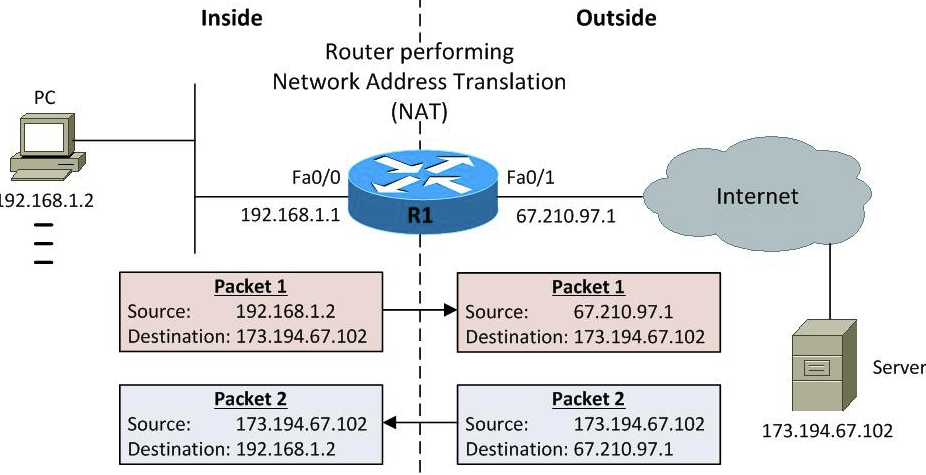
\includegraphics[width=0.7\textwidth]{images/nat}
    \label{fig:LABEL}
\end{figure}

\section*{How does NAT maintain NAT table?}

\begin{itemize}
	\item It creates a table entry \textcolor{blue}{on-the-fly} (automatically) i.e. when client on the internal network contacts server on external network
	\item chooses a NAT port that does \textcolor{red}{not} create \textcolor{red}{collision} in the table
\end{itemize}

\section*{Servers Behind a NAT need \textcolor{red}{port forwarding}}

\begin{itemize}
	\item \textbf{Problem}: Assume A runs a server at TCP port 5000; automatic operation of NAT requires communication to be started by A, which is not done for a server (it doesn't issue requests by itself)
	\item \textbf{Solution}: \textcolor{red}{manual configuration} of port forwarding in NAT
	\begin{itemize}
		\item client connects to server at 54.32.105.4:443
		\item Server needs to know its NAT IP address in advance and advertise it to potential clients 
		\item Server can discover its NAT IP address via STUN server or UPnP (if the server and the NAT use it)
	\end{itemize}
		
	\item \textbf{Side benefit}: \textcolor{blue}{protection}; a server port is accessed only if explicitly configured, while other ports remain unreachable. 
\end{itemize}

% Quick centered image
\begin{figure}[H]
    \centering
    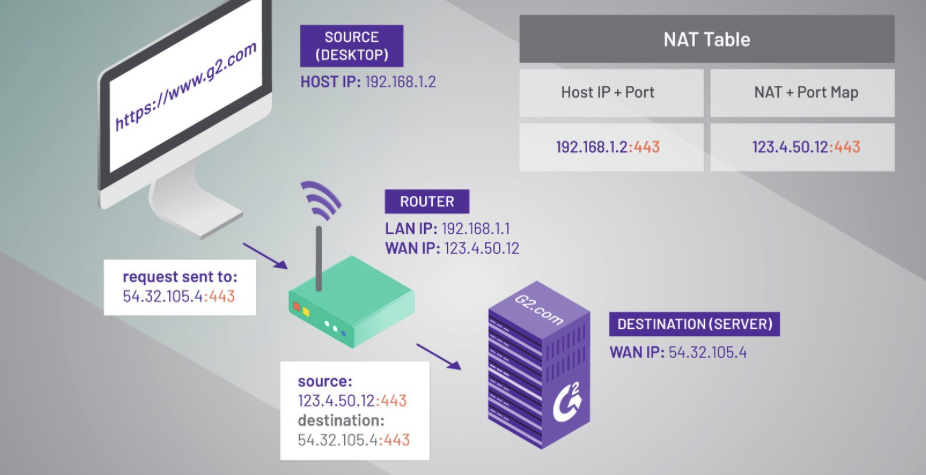
\includegraphics[width=0.8\textwidth]{images/natserver}
    \label{fig:LABEL}
\end{figure}

\section*{NATs and IPv6}

Recall: NAT was motivated by lack of IPv4 addresses. But in IPv6, home routers often: 
\begin{itemize}
	\item \textcolor{red}{do not use NAT},
		\begin{itemize}
			\item their provider typically allocates \textcolor{blue}{a block of IPv6 addresses} not just one as in IPv4
		\end{itemize}
	\item provide protection by acting as a \textcolor{blue}{filtering router}, which:
		\begin{itemize}
			\item allows communication from outside, only if initiated from inside, unless manually configured
		\end{itemize}
	\item Some systems still use NAT with IPv6, if local network receives \textcolor{red}{only one IPv6} address, not an entire prefix
	\item \textcolor{red}{How?}
		\begin{itemize}
			\item Use \textcolor{blue}{link local IPv6 addresses} for internal network $\Rightarrow$ the internal network is a  \textcolor{blue}{single LAN} (only one subnet)
		\end{itemize}
				
	\item Typical case in virtualization e.g. Virtual Box ("NAT network")
\end{itemize}

\section*{Carrier-Grade NAT (CG NAT)}
% Quick centered image
\begin{figure}[H]
    \centering
    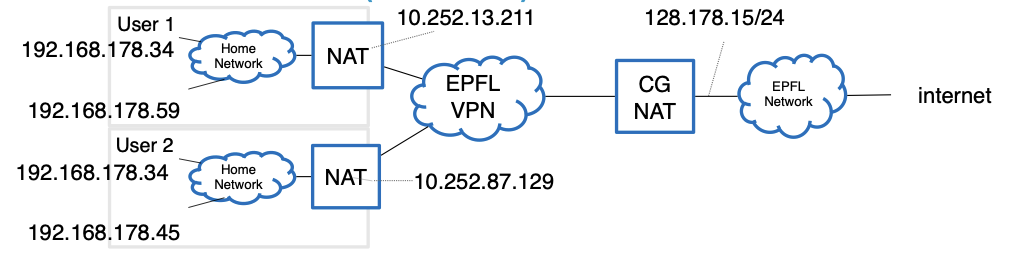
\includegraphics[width=0.7\textwidth]{images/gcnat}
    \label{fig:LABEL}
\end{figure}

\textcolor{red}{What?} Shares \textcolor{red}{p} external/NAT addresses among \textbf{n $>$ p} internal hosts
\begin{itemize}
\begin{itemize}
	\item e.g.: VPN access of EPFL uses the block 128.178.15/24 (i.e p = 256);
	\item VPN user 1 may appear in the public internet with address 128.178.15.x, while VPN user 2 may appear with the same IP address or not
\end{itemize}
\end{itemize}

\begin{itemize}
	\item Some internet service providers use it, in order to \textcolor{blue}{reduce} the number of public \textcolor{blue}{IPv4 addresses} allocated to end-users $\Rightarrow$ they use block  \textcolor{blue}{100.64/10} instead of 10/8
	\item Figure implies \textcolor{red}{"NATs behind NATs"}: 
	\begin{itemize}
		\item e.g. User 1 appears as 192.168.178.34 at home, as 10.252.13.211 at EPFL's VPN and as 128.178.15.x in the public internet
	\end{itemize}
\end{itemize}

\section*{Other NAT types}

% Quick centered image
\begin{figure}[H]
    \centering
    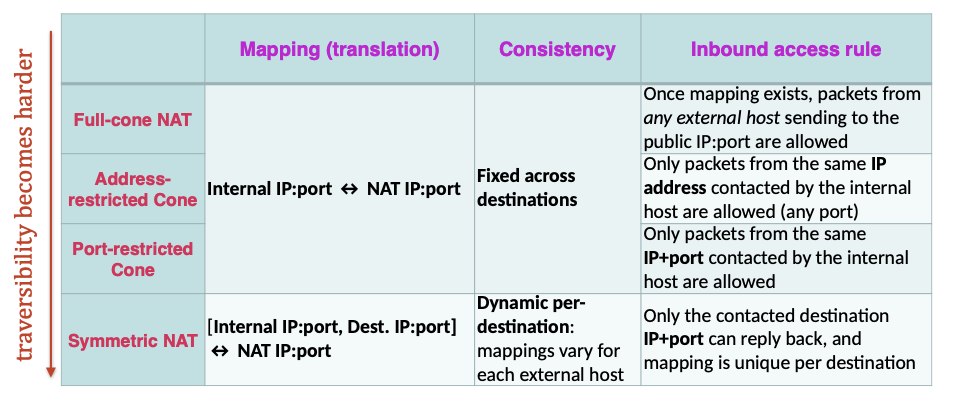
\includegraphics[width=1\textwidth]{images/other-nat-types}
    \label{fig:LABEL}
\end{figure}

\begin{itemize}
	\item ICMP packets don't have port numbers. What to do?
		\begin{itemize}
			\item Some NATs just don't support ICMP; other manipulate the \textcolor{red}{ICMP echo request ID}
		\end{itemize}
\end{itemize}

\begin{itemize}
	\item A \textcolor{red}{full cone NAT} is one where all requests from the same internal IP address+port are \textcolor{red}{always} mapped to the same NAT IP address+port
	\begin{center}
		\textcolor{blue}{(internal addr+port)$\Rightarrow$(NAT addr, NAT port)}
	\end{center}
	So, if the same host sends a packet with the same source address and port, but to a different destination,
a different mapping is used. I.e. same internal IP+port may get multiple different public ports.
Moreover, only the external host that receives a packet can send a packet back to the internal host.
	\item ICMP packets don't have a port number. Some NATs don't support ICMP. Others manipulate e.g. the \textcolor{red}{ICMP echo request identifier} (in ping messages) as a replacement of port number.
\end{itemize}

\begin{tcolorbox}[
  colback=gray!15,     % background color
  colframe=black!50,    % border color
  boxrule=1pt,       % border thickness
  arc=3mm,             % rounded corners
  left=4mm, right=4mm, top=2mm, bottom=2mm % padding
]
\textbf{From WAN to LAN, the typical NAT may modify...}

\vspace{0.3cm}
% Quick centered image
\begin{figure}[H]
    \centering
    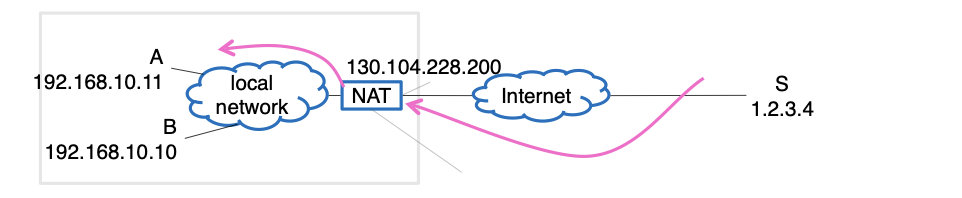
\includegraphics[width=0.8\textwidth]{images/nat-question}
    \label{fig:LABEL}
\end{figure}

\begin{itemize}
	\item A) The source port
	\item B) The destination port
	\item C) None of the above
	\item D) I do not know \\
\end{itemize}

\textbf{Solution:} B
\end{tcolorbox}

\begin{tcolorbox}[
  colback=gray!15,     % background color
  colframe=black!50,    % border color
  boxrule=1pt,       % border thickness
  arc=3mm,             % rounded corners
  left=4mm, right=4mm, top=2mm, bottom=2mm % padding
]
\textbf{When a typical NAT has a packet to forward and an entry exists in the NAT table...}

% Quick centered image
\begin{figure}[H]
    \centering
    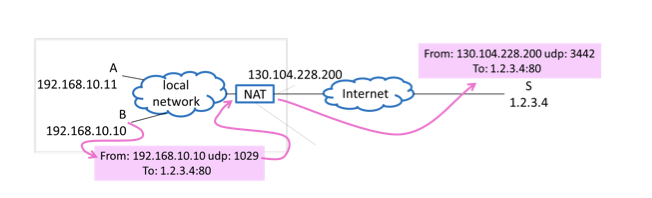
\includegraphics[width=0.6\textwidth]{images/nat-question-2}
    \label{fig:LABEL}
\end{figure}

\vspace{0.3cm}
\begin{itemize}
	\item A) NAT looks the NAT table for a longest prefix match
	\item B) NAT looks the NAT table for an exact matching entry
	\item C) None of the above
	\item D) I do not know \\
\end{itemize}

\textbf{Solution}: B
\end{tcolorbox}

\begin{tcolorbox}[
  colback=gray!15,     % background color
  colframe=black!50,    % border color
  boxrule=1pt,       % border thickness
  arc=3mm,             % rounded corners
  left=4mm, right=4mm, top=2mm, bottom=2mm % padding
]
\textbf{Suppose that the internal subnet uses a private block of
addresses 10.0.0.0/8, what is the max number of internal
hosts (end-systems) that a typical NAT can support?}

% Quick centered image
\begin{figure}[H]
    \centering
    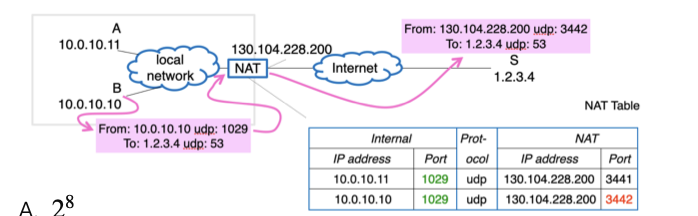
\includegraphics[width=0.7\textwidth]{images/nat-question-3}
    \label{fig:LABEL}
\end{figure}
\vspace{0.3cm}
\begin{itemize}
	\item A) 2^{8}
	\item B) 2^{8} - 1
	\item C) As many as the space of UDP/TCP, 16-bit port numbers (i.e. $\leq 2 \cdot 2^{16} = 2*65536)$
	\item D) None of the above
	\item E) I do not know	\\
\end{itemize}
\textbf{Solution}: C \\
\begin{itemize}
	\item NAT creates table entries on the fly by also trying to avoid collisions on the port number. So, the max
number of entries it can have is equal to the overall number of the TCP/UDP port numbers that it is
allowed to use (i.e. that are not reserved for other purposes and not blocked by a firewall). This number
is smaller than 2*65536, since each port number is 16bits long; hence for each of TCP and UDP, we
have $2^{16}$ = 65536 possible numbers.
	\item The latter is smaller than the overall number of private IP addresses in the allocated block (which is $2^{24}$ addresses, because the subnet mask is /8).
	\item So, it is also the max number of hosts that the NAT can support—the max number of hosts is achieved
by assuming that each host has only one UDP or TCP connection with some other host outside the LAN.
\end{itemize}

\end{tcolorbox}
\section*{5. Configuration of a network interface}

\begin{itemize}
	\item A \textcolor{red}{host} IP interface is configured with:
	\begin{itemize}
		\item IP address of this interface
		\item Subnet mask of this interface
		\item IP address of default gateway router
		\item IP address of DNS server
	\end{itemize}

	\item Can be configured \textcolor{blue}{manually}, or \textcolor{blue}{automatically} with:
		\begin{itemize}
			\item IPv4 DHCP (Dynamic Host Configuration Protocol)
			\item IPv6 DHCP stateful, SLAAC (stateless), DHCP stateless
		\end{itemize}
	\item Same applies to \textcolor{red}{routers} connected to a provider
		\begin{itemize}
			\item IPv4 PPP (Point to Point protocol): automatic config for telecom lines (modem, ADSL)
			\item IPv6 PPP, DHCP with Prefix Delegation
		\end{itemize}
\end{itemize}


\section*{DHCP (Dynamic Host Configuration Protocol)}

\begin{itemize}
	\item \textcolor{blue}{Client-Server} app: configuration info is kept in DHCP server; host contacts the server when it needs an IP address
	\item Common in IPv4; also works with IPv6 (called stateful DHCP)
\end{itemize}

\textbf{Problem}: Host cannot contact the DHCP server since it does not know of \textcolor{red}{any} IP address initially

\textbf{Solution}: Use broadcast (IPv4) or multicast (IPv6) inside the LAN to \textcolor{blue}{discover} DHCP servers

\textbf{Details}:
\begin{itemize}
	\item Either DHCP server exists in the same LAN or gateway router implements a "\textcolor{red}{DHCP Relay}" function
	\item DHCP uses \textcolor{blue}{two phase commit} with acknowledgement to avoid inconsistent reservations
	\item DHCP server keeps \textcolor{blue}{state} for each "lease" (=reservation) -- renews leaser after expiry
\end{itemize}

Example (IPv4):

% Quick centered image
\begin{figure}[H]
    \centering
    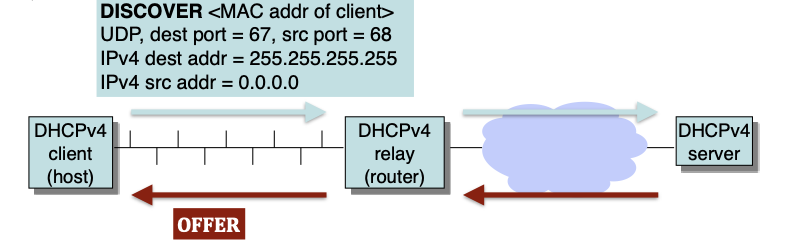
\includegraphics[width=0.9\textwidth]{images/dhcp}
    \label{fig:LABEL}
\end{figure}
\section*{(Self)-Autoconfiguration in IPv4}

\begin{itemize}
	\item \textcolor{red}{Why?} If \textcolor{red}{no DHCP} is available and \textcolor{red}{no manual} configuration is done
\end{itemize}

\begin{itemize}
	\item \textcolor{red}{What it does?} Enables interconnection in unmanaged or "router-less" local networks, but not in a general setting
\end{itemize}

\begin{itemize}
	\item \textcolor{red}{How?} When a host boots, it: 
	\begin{itemize}
		\item 1. picks an IPv4 link local address \textcolor{blue}{at random} in block \textcolor{blue}{169.254/16}
		\item 2. performs an \textcolor{blue}{address duplication test} using \textcolor{red}{broadcast} IP
	\end{itemize}
	\item Implemented in Windows, not always supported in Linux
\end{itemize}


\section*{Stateless Address \textcolor{purple}{Auto}configuration (SLAAC) in IPv6}

\textcolor{red}{Why} invented? To configure interfaces automatically without DHCP servers in IPv6

\textcolor{red}{How} it works?
\begin{itemize}
	\item 1. Host auto-configures a \textcolor{blue}{link local address} with a 64-bit \textcolor{red}{prefix} (fe80::/64) + a 64-bit \textcolor{red}{host suffix} that is derived by one of the following:
	\begin{itemize}
		\item (i) manually, e.g. ::1
		\item (ii) algorithmically from MAC address (“\textcolor{blue}{modified EUI 64"})
		\item (iii) randomly (\textcolor{blue}{temporary} validity) 
		\item (iv) via \textcolor{blue}{“secure autoconf”} (RFC7217), i.e. randomly but also related to subnet 
		\item (v) cryptographically with CGA
	\end{itemize}
	\item 2. host performs \textcolor{blue}{address duplication test} using \textcolor{red}{solicited node multicast} address (which has the same 24 last bits as the address it has selected)
		(see image for reserved address blocks for IPv6)
	\item 3. host computes globally valid address by obtaining the network prefix from LAN's router (via \textcolor{red}{multicasting})
\end{itemize}

$\Rightarrow$ SLAAC is fully  \textcolor{blue}{automatic} but does \textcolor{red}{not} provide DNS information

\section*{Random and RFC7217 Addresses avoid Host Tracking}

Solution 1: \textcolor{blue}{temporary, random host suffix}

% Quick centered image
\begin{figure}[H]
    \centering
    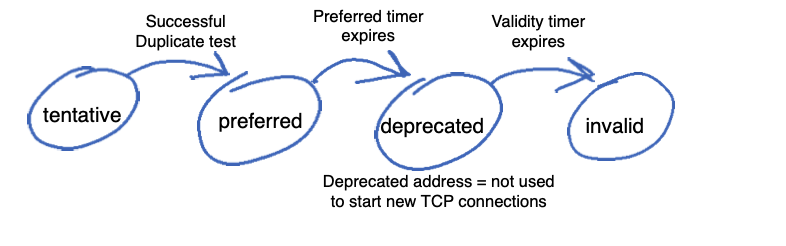
\includegraphics[width=0.8\textwidth]{images/host-tracking}
    \label{fig:LABEL}
\end{figure}

Solution 2: "\textcolor{blue}{Secure autoconf}" (RFC7217), not fully random but \textcolor{blue}{intractable} host suffix:
\begin{center}
\textcolor{red}{\verb|Host suffix = hash (interface id, subnet prefix, secret key)|} 
\begin{itemize}
	\item Key is obtained with OS installation
	\item Address remains the same whenever host visits same subnet
	\item Address changes randomly accross different subnets
\end{itemize}

\end{center}
\section*{How to learn IP of DNS (after SLAAC)?}

\begin{itemize}
	\item Stateless DHCP
	\begin{itemize}
		\item gives the IP address of the DNS server to the host
	\item does not keep state for IP leases
\end{itemize}
	
\end{itemize}

\begin{itemize}
	\item Router Advertisements (RFC 6106)
	\begin{itemize}
		\item Host accesses routers in the same LAN via \textcolor{blue}{multicasting} asking for DNS info
	\item Router returns the IP address of the DNS server to the host
\end{itemize}
	
\end{itemize}

\section*{DHCP with Prefix Delegation}

\textcolor{red}{Why?} A home (or enterprise) IPv6 router is configured by ISP using DHCP; local devices are autoconfigured using e.g. SLAAC.

And home router needs to advertize an IPv6 prefix for the \textcolor{red}{entire} home network

\textcolor{red}{How?}
\begin{itemize}
	\item ISP DHCP server (delegating router) provides the home router with not just a single IPv6 address but also the network prefix that this router can \textcolor{blue}{\textit{delegate}} to its devices
	\item  If the prefix used for the link from ISP to the home router is a subset of the delegated prefix, then it is \textcolor{red}{\textit{excluded}} from the delegation (RFC 6603). \\
E.g. 2004:aaaa:bbbb:cc01/64 is excluded from the delegated prefix 2004:aaaa:bbbb:cc01/60.
\end{itemize}

% Quick centered image
\begin{figure}[H]
    \centering
    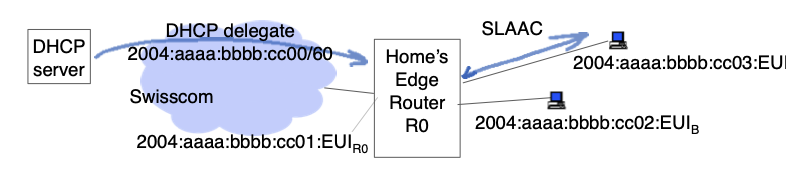
\includegraphics[width=0.8\textwidth]{images/dhcp-prefix-del}
    \label{fig:LABEL}
\end{figure}

\textbf{Question}: \textcolor{blue}{When an IPv4 host uses DHCP, which of the following information
does it acquire?}

\textcolor{blue}{1. Its own IP address}

\textcolor{blue}{2. A subnet mask related to the subnet it belongs to}

\textcolor{blue}{3. The address of the default gateway}

\textcolor{blue}{4. The address of the DNS server}

\begin{itemize}
	\item A) 1
	\item B) 1, 2
	\item C) 1, 2, 3
	\item D) 1, 2, 3, 4
	\item E) None of the above
\end{itemize}

\textbf{Solution}: D

\begin{tcolorbox}[
  colback=gray!15,     % background color
  colframe=black!50,    % border color
  boxrule=1pt,       % border thickness
  arc=3mm,             % rounded corners
  left=4mm, right=4mm, top=2mm, bottom=2mm % padding
]
\textbf{With SLAAC an IPv6 host has…}

\vspace{0.3cm}

\begin{itemize}
	\item A) A link local address and, if a router is present in the subnet, also a global unicast address
	\item B) If a router is present in the subnet a global unicast address and no link-local address
	\item None of the above
	\item I do not know \\
\end{itemize}

\textbf{Solution}: A
\end{tcolorbox}
\section*{Private vs link local addresses}

Private addresses are allocated \textcolor{red}{administratively} (i.e., by a local network administrator, either statically, or automatically allocated at a single point by a suitably configured DHCP server).

Link-local addresses are allocated \textcolor{red}{automatically} (e.g. via SLAAC) when a computer has not been configured with a static IP-address and cannot find a DHCP server.

\begin{itemize}
	\item Why do we need a \textcolor{blue}{separate space} for link local?
\end{itemize}
So that the link-local addresses cannot possibly conflict with those allocated by a local, but temporarily unavailable, DHCP server.

\begin{itemize}
	\item How are link local and private addresses handled by gateway routers?
\end{itemize}

They are not routed. This is so that lots of private LANs can use the same addresses without any routing conflicts arising. Such LANs must use NAT to hide their many private addresses behind one (or a few) public addresses.

\begin{itemize}
	\item Can both interfaces of a gateway router/NAT (internal and external) be configured with private addresses?
\end{itemize}

Yes, but they cannot belong to the same subnet. We use a different subnet at each “side” of the router/NAT.

\section*{6. Revisit IP Header: Hop Limit (HL) / Time to Live (TTL)}
\textcolor{red}{Why?} avoid looping packets in transient loops. Transient loops may exist due to change to forwarding tables + propagation latency. 

% Quick centered image
\begin{figure}[H]
    \centering
    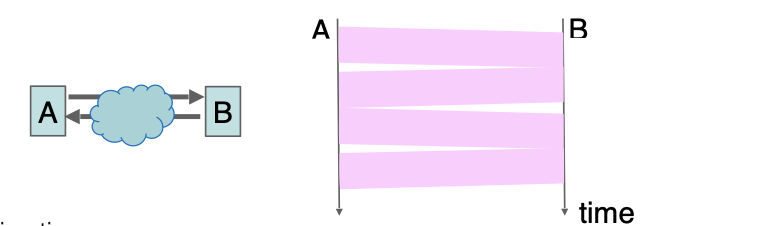
\includegraphics[width=0.6\textwidth]{images/ip-header}
    \label{fig:LABEL}
\end{figure}

If propagation time is small compared to transmission time, a single packet (or a few packages) caught in a loop can congest the line. 

\textcolor{red}{How?}
\begin{itemize}
	\item Every IP packet has a field on 8 bits (from 0 to 255) (called Hop Limit in IPv6 / Time To Live in IPv4) that is decremented at every IP hop
	\item Every router or NAT decreases HL/TTL, switches do \textcolor{red}{not}
	\item When HL/TTL reaches 0, packet is discarded
	\item At source, value is 64 in principle
\end{itemize}

\section*{Traceroute leverages the HLs/TTLs}

\begin{itemize}
	\item It sends a series of packets (using UDP) to a destination, with TTL = 1, 2, 3, ...
	\item Routers on the path discard packets and send ICMP error message back to source
	\item Source learns address of router on the path by looking at source address of error message
	\item tracert (windows) is similar, but uses ICMP
\end{itemize}

\textbf{Checksum}

\begin{itemize}
	\item IPv4 only, protects header against bit errors
	\item \textcolor{red}{absent in IPv6} (layer 2 and router hardware assumed to have efficient error detection)
\end{itemize}

\begin{tcolorbox}[
  colback=gray!15,     % background color
  colframe=black!50,    % border color
  boxrule=1pt,       % border thickness
  arc=3mm,             % rounded corners
  left=4mm, right=4mm, top=2mm, bottom=2mm % padding
]
\textbf{A host generates a packet with Hop Limit = 1}

\vspace{0.3cm}

\begin{itemize}
	\item A) This packet is invalid
	\item B) This packet will never be forwarded by a switch nor by a router
	\item C) This packet will never be forwarded by a switch but may be forwarded by a router
	\item D) This packet will never be forwarded by a router but may be forwarded by a switch
	\item E) None of the above is true
	\item F) I do not know \\
\end{itemize}

\textbf{Solution}: D \\

This packet cannot be forwarded by a router because it would
decrement the HL and obtain 0. It can be forwarded by a switch
because a switch does not examine the IP header. \\
Note that such a packet is perfectly valid. Sources put HL=1 when
they want to be sure that the packet remains in the LAN.

\end{tcolorbox}
\end{document}
